Il presente capitolo è dedicato all'analisi dei risultati ottenuti applicando la pipeline descritta nel Capitolo 3 e al confronto tra i diversi approcci e algoritmi considerati. Al fine di evitare ridondanze, in questa sezione vengono riportate esclusivamente le informazioni necessarie all'interpretazione dei risultati sperimentali, mentre i dettagli metodologici relativi al rigging, allo skinning e al retargeting automatico sono stati già discussi nei capitoli precedenti.

Gli esperimenti sono stati condotti su oggetti 3D inanimati e non antropomorfi, utilizzando le stesse animazioni di input per tutti gli approcci, così da garantire condizioni di confronto omogenee. I risultati sono presentati principalmente sotto forma di confronti visivi e di una valutazione quantitativa basata su una metrica di errore definita ad hoc, finalizzata a misurare il grado di discostamento da un risultato ritenuto ottimale.

Nelle successive vengono analizzati separatamente i risultati delle diverse fasi di pipeline (rigging, skinning e retargeting) e viene infine fornito un confronto complessivo tra gli approcci considerati.

\section{Risultati del rigging automatico}

In questa sezione vengono presentati i risultati ottenuti nella fase di rigging automatico applicando gli approcci UniRig e RigAnything agli oggetti 3D inanimati descritti nel Capitolo 3.
Sono stati considerati esclusivamente questi due metodi in quanto entrambi includono una fase di generazione automatica dello scheletro a partire della mesh, rendendo possibile un confronto diretto.

Per ciascun oggetto, il rig generato è stato analizzato dal punto di vista del posizionamento delle ossa, della coerenza strutturale con la geometria della mesh e della copertura delle parti articolabili.

\subsection{Confronto visivo del rigging}

\begin{figure}[h]
\centering
\begin{subfigure}{0.45\textwidth}
    \centering
    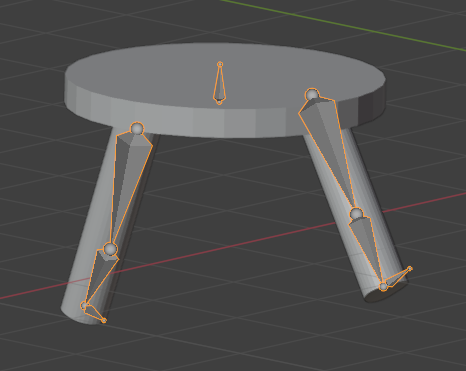
\includegraphics[width=\linewidth]{figure/rigging.png}
    \caption{Rigging generate da UniRig}
\end{subfigure}
\hfill
\begin{subfigure}{0.45\textwidth}
    \centering
    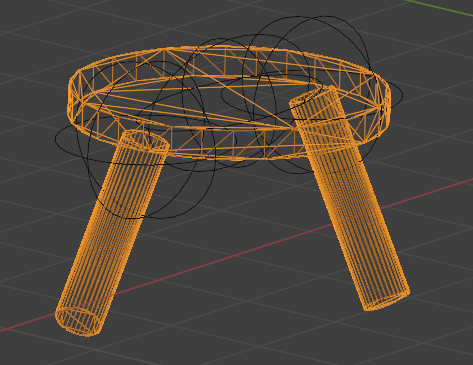
\includegraphics[width=\linewidth]{figure/wireframe.png}
    \caption{Rigging generate da RigAnything}
\end{subfigure}
\caption{Risultato del rigging automatico}
\label{fig:rigging}
\end{figure}

La figura ~\ref{fig:rigging} mostra il confronto visivo tra le strutture di rigging generate da UniRig e RigAnything sul modello del piatto con due gambe. Nel caso di UniRig, lo scheletro generato è rappresentato da un'armature esplicita, con ossa chiaramente allineate alle principali componenti strutturali dell'oggetto, in particolare alle due gambe e alla poszione centrale del piatto.

Per RigAnything, la struttura di controllo non è espressa tramite un'armature tradizionale, ma attraverso controlli impliciti che guidano la deformazione della mesh. Tali controlli sono visualizzati medianti punti di controllo sovrapposti alla mesh e tramite la visualizzazione wireframe, evidenziandole regioni soggette a movimento.

\subsection{Analisi qualitativa}
L'analisi qualitativa dei risultati evidenzia come UniRig e RigAnything adottino strategie differenti nella fase di rigging automatico, ottimizzando aspetti diversi del problema.

Dal punto di vista strutturale, UniRig genera un'armatura esplicita, semanticamente interpretabile e direttamente utilizzabile all'interno delle pipeline di animazione tradizionali basati su scheletri. La presenza di ossa chiaramente definite facilita le successive fasi di skinning e retargeting , risultando particolarmente vataggiosa in contesti in cui è richiesto un controllo esplicito della struttura dell'oggetto.

RigAnything, invece, non produce uno scheletro esplicito, ma utilizza una struttura di controllo implicita che privilegia la stabilità della deformazione della mesh. Questo approccio consente una maggiore flessibilità nel tratamento di geometrie non antropomorfe, ma riduce l'interpretabilità del rig e la sua integrazione diretta con strumenti di animazione scheletrica standard.

In sintesi, UniRig risulta più adatto a scenari in cui è richiesta una rappresentazione strutturale chiara del rig, mentre RigAnything mostra vantaggi nella gestione della deformazione, sopratutto in presenza di geometrie articolate e non convenzionali. Nessuno dei due approcci risulta pertanto globalmente superiore, ma ciascuno presenta punti di forza specifici in funzione del criterio di valutazione considerato.

\section{Risultato dello skinning}

In questa sezione vengono analizzati i risultati ottenuti nella fase di skinning automatico valutando la qualità delle deformazioni prodotte durante l'animazione degli oggetti 3D. Lo skinning è stato applicato agli scheletri e alle strutture di controllo generati nella fase di rigging, mantenendo invariata l'animazione di input per tutti gli approccii.

\subsection{Confronto visivo delle deformazioni}

\begin{figure}[H]
\centering
\begin{subfigure}{0.45\textwidth}
    \centering
    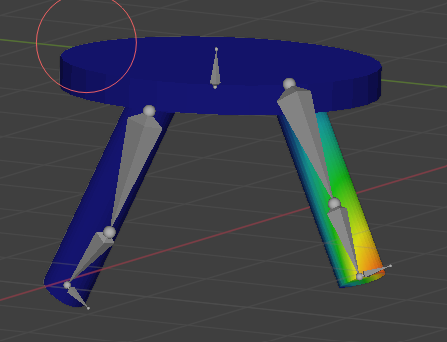
\includegraphics[width=\linewidth]{figure/skinning.png}
    \caption{Skinning generate da UniRig}
\end{subfigure}
\hfill
\begin{subfigure}{0.45\textwidth}
    \centering
    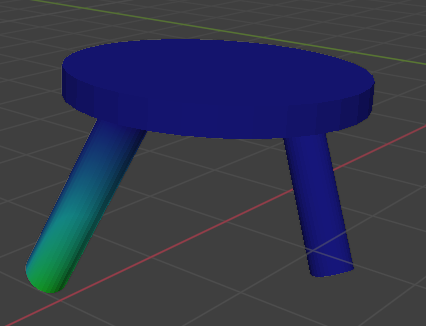
\includegraphics[width=\linewidth]{figure/peso.png}
    \caption{Skinning generate da RigAnything}
\end{subfigure}
\caption{Risultato dello skinning automatico}
\label{fig:skinning}
\end{figure}

La figura ~\ref{fig:skinning} mostra un confronto visivo delle deformazioni ottenute applicando lo skinning automatico ai rig generati da UniRig e RigAnything sul modello del piatto con due gambe, in corrispondenza di frame rappresentativi dell'animazione.

Nel caso di UniRig, la deformazione della mesh risulta coerente con la struttura scheletrica esplicita, ma sono visibili lievi artefatti locali in prossimità delle giunzioni tra le gambe e il piatto, dovuti alla distribuzione dei pesi di influenza sui vertici.

Per RigAnything, la deformazione appare più uniforme lungo le parti articolate, con una riduzione degli artefatti locali nelle regioni di maggiore movimento. Tuttavia, la mancanza di una struttura ossea esplicita rende meno inmediata l'individuazione delle regioni di controllo responsabili della deformazione.

\subsection{Analisi qualitativi dello skinning}

L'analisi quantitativa evidenzia come la qualità dello skinning sia fortemente influenzata dalla struttura di rigging sottostante.

Nel caso di UniRig, la presenza di un'armature esplicita consente una chiara associazione tra ossa e regioni della mesh, facilitando il controllo della deformazione e l'eventuale intervento correttivo. Tuttavia, lo skinning automatico risulta più sensibile alla complessità geometrica, mostrando artefatti locali in corrispondenza di giunzioni non perfettamente allineate alla struttura scheletrica.

RigAnything, utilizzando una struttura di controllo implicita, privilegia la stabilità complessiva della deformazione, producendo risultati visivamente più uniformi nelle regioni articolate. Questo approccio riduce la presenza di collassi locali e stretching eccessivo, ma sacrifica parzialmente l'interpretabilità del processo di skinning.

In sintesi, UniRig offre un maggiore controllo strutturale dello skinning, risultando vantaggioso in scenari in cui è richiesta un'animazione scheletrica tradizionale, mentre RigAnything mostra una maggiore robustezza nella deformazione automatica di oggetti 3D non antropomorfi.

\section{Risultato del retargeting delle animazioni}

In questa sezione vengono analizzati i risultati ottenuti nella fase di retargeting delle animazioni, valutando la capacità dei diversi approcci di trasferire correttamente il movimento da una sorgente animata a oggetti 3D inanimati.
Le animazioni di input, provenienti da Mixamo o MoveAI, sono state applicate utilizzando la stessa pipeline per tutti i metodi, così da garantire condizioni di confronto omogenee.

\subsection{Confronto visivo del retargeting}

\begin{figure}[H]
\begin{center}
     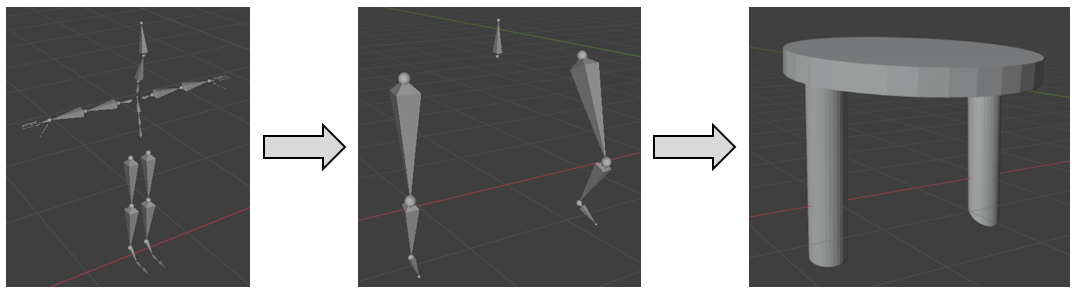
\includegraphics[width=13cm]{figure/processo.png}
     \caption{Frame rappresentativo del risultato di retargeting dell’animazione sull’oggetto target ottenuto con UniRig} 
     \label{fig:cop}
\end{center}
\end{figure}

La figura~\ref{fig:cop} mostra un confronto visivo del retargeting dell'animazione sul modello del piatto con due gambe, in corrispondenza di frame rappresentativi del movimento.

Nel caso di UniRig, il retargeting risulta coerente con la struttura scheletrica esplicita generata nella fase di rigging. Il movimento delle gambe segue in modo interpretabile l'animazione sorgente, mantenendo una chiara corrispondenza tra ossa sorgente e ossa target. Tuttavia, in alcuni frame sono osservabili limitazioni nella naturalezza del movimento, dovute alla rigidità imposta dalla struttura scheletrica.

Per RigAynything, il movimento risulta più fluido e continuo lungo le parti articolate dell'oggetto, con una riduzione delle discontinuità temporali. Tuttavia, l'assenza di una mappatura scheletrica esplicita rende meno immediato il controllo semantico del movimento e la sua modifica manuale.

\subsection{Analisi qualitativa}

L'analisi qualitativa dei risultati evidenzia come la fase di retargeting sia fortemente influenzata dalle scelte effettuata nelle fasi di rigging e skinning.

Tali differenze emergono in modo evidente anche dall'analisi qualitativa delle traiettorie dei punti articolari equivalenti, riportate nei grafici seguenti, in cui è possibile osservare un comportamento più regolare e strutturalmente coerente nel caso di UniRig rispetto a un andamento più fluido ma meno controllabile nel caso di RigAnything.

\begin{figure}[H]
\begin{center}
     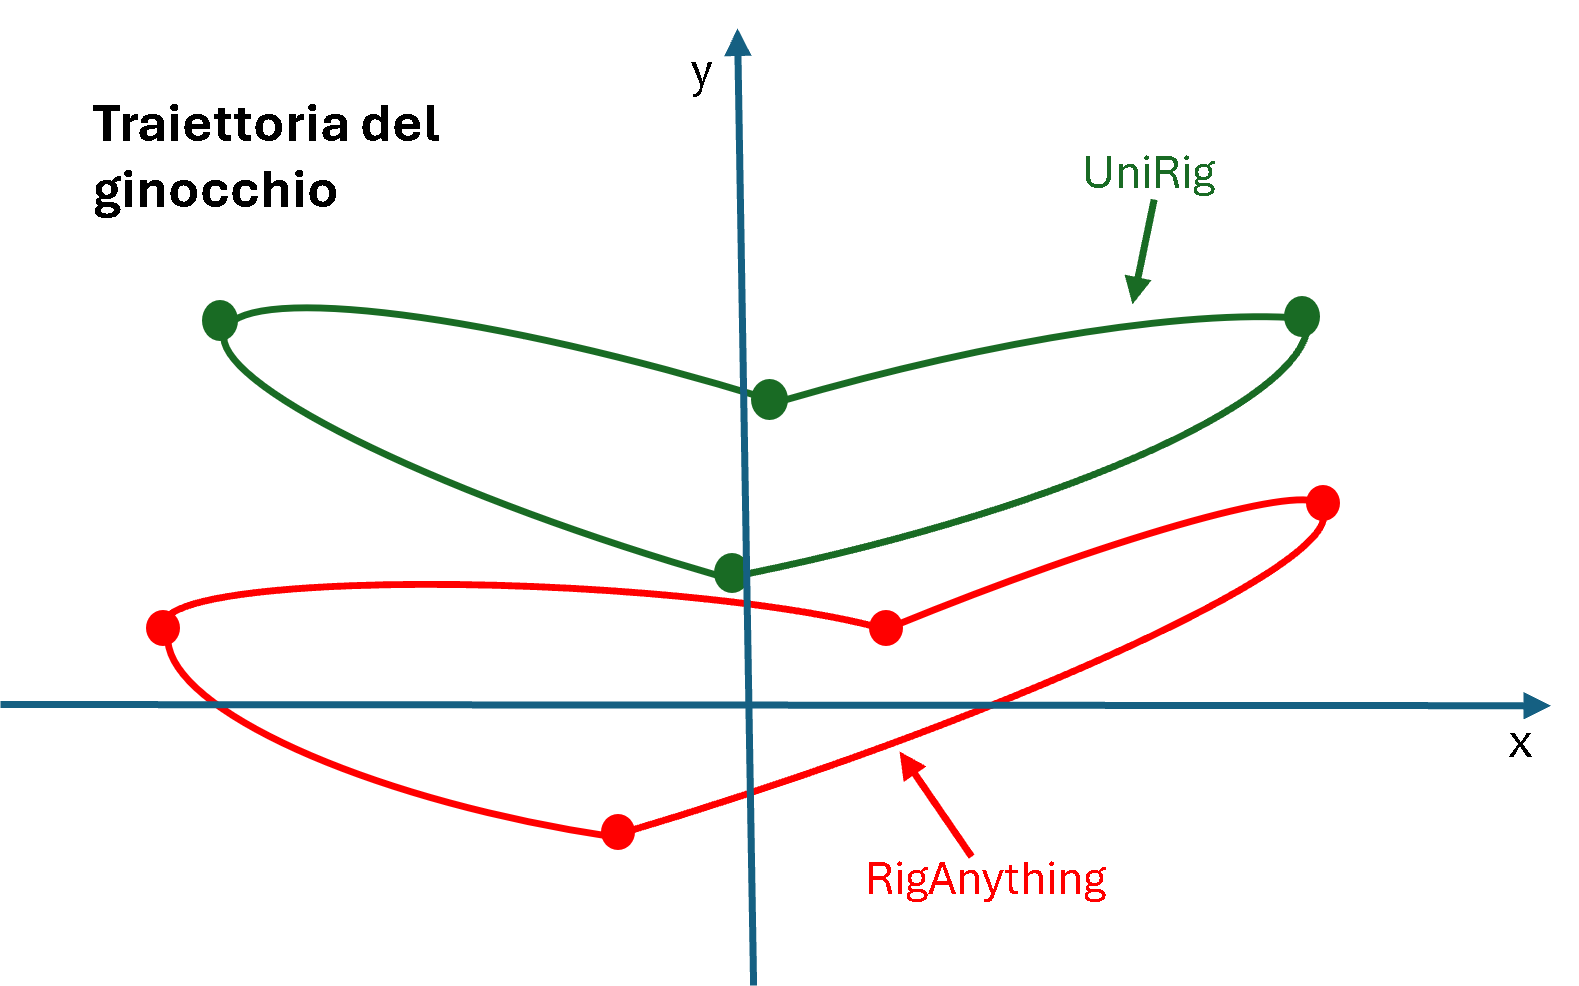
\includegraphics[width=13cm]{figure/ginocchio.png}
     \caption{Rappresentazione qualitativa delle traiettorie del punto articolare intermedio (equivalente al ginocchio) durante il retargeting dell’animazione, proiettate su un piano bidimensionale.}
     \label{fig:tab}
\end{center}
\end{figure}

\begin{figure}[H]
\begin{center}
     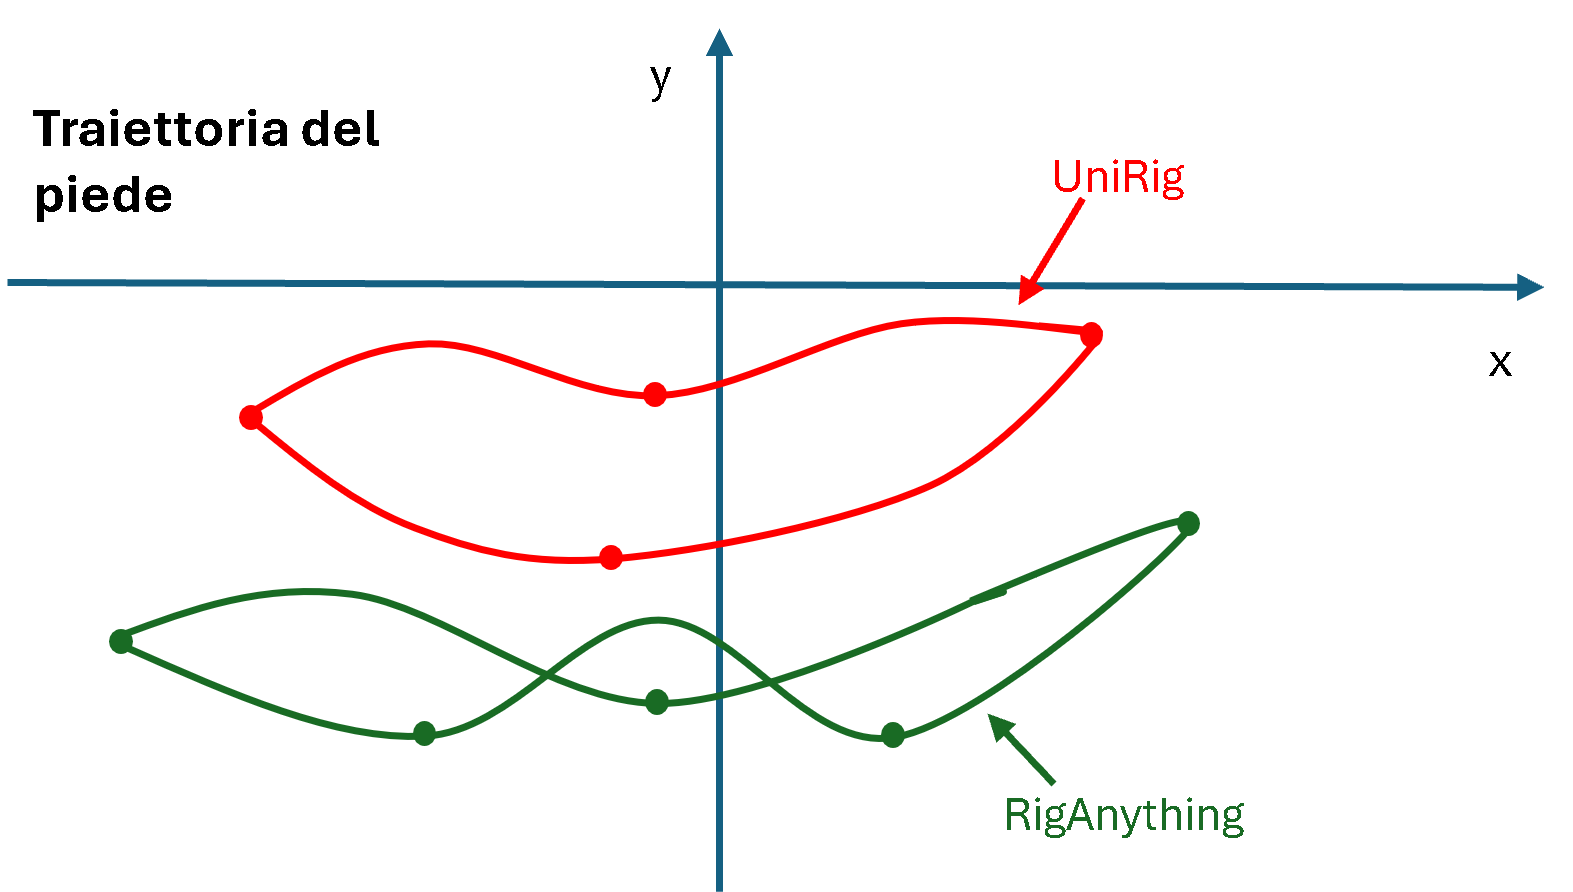
\includegraphics[width=13cm]{figure/piede.png}
     \caption{Rappresentazione qualitativa delle traiettorie del punto terminale della gamba (equivalente al piede) durante il retargeting dell’animazione.}
     \label{fig:tab}
\end{center}
\end{figure}

UniRig, grazie alla presenza di un'armature esplicita, cosente un retargeting più diretto e semanticamente coerente con le animazioni sorgente, risultando particolarmente adatto a pipeline basate su scheletri standard. Questa caratteristica facilita il trasferimento di animazioni provenienti da dataset antropomorfi, come Mixamo, anche su oggetti non convenzionali.

RigAnything, invece, mostra una maggiore flessibilità nel trasferimento del movimento, adattando l'animazione alla geometria dell'oggetto senza richiedere una corrispondenza scheletrica rigida. Questo approccio produce movimenti visivamente più fluidi, ma rende più complesso il controllo fine del retargeting e la sua riproducibilità su animazioni differenti.

In sintesi, UniRig risulta più indicato in scenari in cui è richiesta una corrispondenza strutturale tra animazioni sorgente e target, mentre RigAnything privilegia la qualità visiva del movimento adattato, a scapito della controllabilità semantica.

\subsection{Confronto con altri approcci}

Oltre al confronto sperimentale diretto tra UniRig e RigAnything, i risultati ottenuti sono stati messi in relazione con alcuni approcci rappresentativi presenti in letteratura, tra cui ASMR, AnyTop e NOR (Neural Object Rigging).
Poiché tali metodi non sono stati implementati e testati direttamente nel presente lavoro, il confronto è stato condotto su base metodologica e qualitativa, facendo riferimento alle caratteristiche dichiarate e ai risultati riportati nei rispettivi lavori.

Gli approcci considerati differiscono significativamente per quanto riguarda la rappresentazione del rig, la gestione dello skinning e il supporto al retargeting delle animazioni. In particolare, ASMR si basa su una struttura scheletrica esplicita e su una corrispondenza rigida tra sorgente e target, risultando maggiormente orientato a modelli antropomorfi. AnyTop e NOR, invece, adottano strategie più flessibili, mirate al trattamento di geometrie generiche e non convenzionali, ma presentano un supporto limitato o parziale al retargeting di animazioni complesse.

Nel contesto del presente lavoro, UniRig e RigAnything si collocano come approcci intermedi tra i metodi puramente scheletrici e quelli completamente impliciti. UniRig condivide con ASMR l’uso di un’armature esplicita, facilitando il retargeting semantico delle animazioni, ma estende tale paradigma a oggetti non antropomorfi. RigAnything, invece, si avvicina maggiormente ad approcci come AnyTop e NOR, privilegiando l’adattamento del movimento alla geometria dell’oggetto e la qualità visiva del risultato finale, a scapito della controllabilità strutturale. Questo confronto si vede più chiaramente nella seguente figura ~\ref{fig:tab}.

\begin{figure}[H]
\begin{center}
     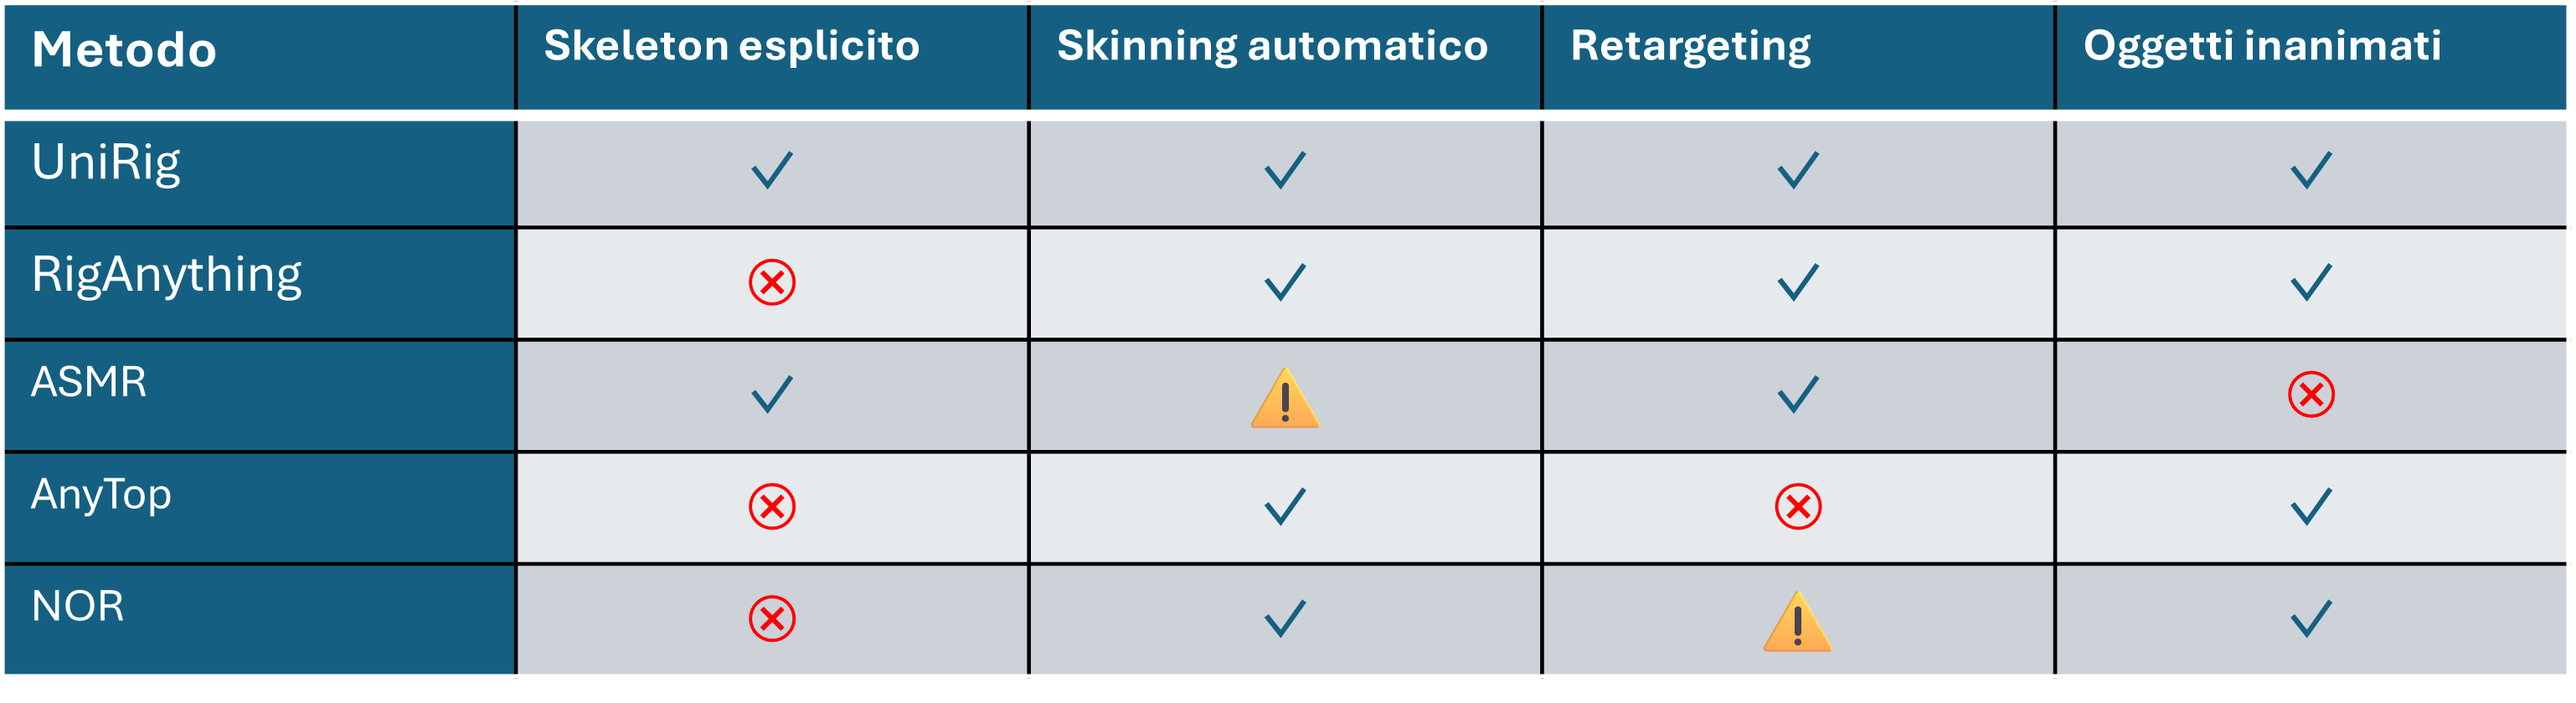
\includegraphics[width=13cm]{figure/tabella.png}
     \caption{Confronto qualitativo tra i diversi approcci, evidenziandone punti di forza e limitazioni nel contesto del retargeting di animazioni su oggetti 3D}
     \label{fig:tab}
\end{center}
\end{figure}

\section{Definizione della metrica di errore}

\subsection{Motivazioni e obbiettivi}

La valutazione dei risultati ottenuti mediante tecniche di rigging automatico, skinning e retargeting di animazioni su oggetti 3D inanimati risulta particolarmente complessa, in quanto non esiste un riferimento univoco che definisca una soluzione ottimale. La qualità del risultato dipende infatti da molteplici fattori, tra cui la coerenza strutturale del rig, la stabilità delle deformazioni e la fedeltà del movimento trasferito.
Alla luce di tali considerazioni, è stata definita una metrica di errore composita, con l’obiettivo di quantificare in modo coerente il grado di discostamento del risultato ottenuto rispetto a una soluzione ritenuta ottimale nel contesto applicativo considerato. La metrica proposta consente di confrontare approcci basati su paradigmi differenti, pur mantenendo una valutazione uniforme.

\subsection{Definizione della metrica}

La metrica di errore proposta, denominata \textbf{Composite Retargeting Error} (CRE), è definita come una combinazione pesata di quattro componenti principali:

\begin{align*}
    CRE = {w_s}E_s + {w_d}E_d + {w_t}E_t + {w_c}E_c
\end{align*}

dove ${E_s, E_d, E_t}$ ed ${E_c}$ rappresentano rispettivamente l’errore strutturale, l’errore di deformazione, l’errore temporale e l’errore di controllabilità, mentre ${w_s, w_d, w_t}$ e ${w_c}$ sono i pesi associati a ciascuna componente, tali che:

\begin{align*}
    w_s + w_d + w_t + w_c = 1
\end{align*}

Ciascuna componente è normalizzata nell’intervallo [0,1], dove il valore 0 indica una soluzione ottimale rispetto al criterio considerato, mentre il valore 1 rappresenta una forte deviazione dalla soluzione desiderata.

\subsection{Componenti della metrica}

\textbf{Errore strutturale(${E_s}$)}

L’errore strutturale misura il grado di coerenza del rig generato rispetto a una struttura scheletrica semanticamente interpretabile. In particolare, vengono valutati la presenza di uno scheletro esplicito, la coerenza tra ossa e parti dell’oggetto e la stabilità della gerarchia del rig.
Valori ridotti di ${E_s}$ indicano una struttura facilmente interpretabile e controllabile, mentre valori elevati sono associati a rig impliciti o difficilmente modificabili.

\textbf{Errore di deformazione(${E_d}$)}

L’errore di deformazione quantifica la qualità delle deformazioni della mesh durante l’animazione, tenendo conto di fenomeni quali stretching eccessivo, collassi locali e intersezioni geometriche. La valutazione è stata condotta mediante analisi visiva dei risultati e, ove disponibile, mediante l’osservazione delle mappe di peso associate allo skinning.

\textbf{Errore temporale(${E_t}$)}

L’errore temporale misura la coerenza del movimento nel tempo, considerando la presenza di discontinuità, jitter o perdita di fluidità nel passaggio tra pose successive. La valutazione è stata effettuata su frame rappresentativi dell’animazione, selezionati in corrispondenza di pose significative.

\textbf{Errore di controllabilità(${E_c}$)}

L’errore di controllabilità valuta il grado di accessibilità e modificabilità del risultato ottenuto. In particolare, vengono considerate la possibilità di intervenire manualmente sul rig, la chiarezza del controllo offerto all’utente e la riutilizzabilità dell’animazione su modelli differenti.

\subsection{Applicazione della metrica ai metodi sperimentati}

La metrica di errore è stata applicata ai metodi UniRig e RigAnything, per i quali sono stati ottenuti risultati sperimentali nello stesso contesto applicativo. I valori riportati sono il risultato di una valutazione qualitativa normalizzata, basata sull’analisi visiva dei risultati e sui criteri definiti in precedenza.

\begin{table}[h]
\centering
\caption{Confronto dei valori della metrica di errore per i metodi sperimentati}
\label{tab:cre_methods}
\begin{tabular*}{\textwidth}{@{\extracolsep{\fill}}lccccc}
\hline
\textbf{Metodo} & $\mathbf{E_s}$ & $\mathbf{E_d}$ & $\mathbf{E_t}$ & $\mathbf{E_c}$ & \textbf{CRE} \\
\hline
UniRig      & 0.2 & 0.4 & 0.3 & 0.2 & 0.28 \\
RigAnything & 0.6 & 0.2 & 0.2 & 0.6 & 0.40 \\
\hline
\end{tabular*}
\end{table}

\subsection{Discussione}

L’analisi condotta mediante la metrica proposta evidenzia come gli approcci basati su uno scheletro esplicito tendano a favorire la controllabilità e la coerenza strutturale, mentre i metodi a controllo implicito mostrano generalmente migliori prestazioni in termini di deformazione e adattabilità geometrica. Tali risultati confermano l’assenza di una soluzione globalmente ottimale e sottolineano la presenza di compromessi tra i diversi criteri considerati.
